\section{LP10 Induction électromagnétique}

\begin{header}
\begin{tabular}{p{0.4\textwidth} l}
\niveau & \prerequis \\
Licence & \textbullet{} Electrocinétique \\
        & \textbullet{} Forces de Laplace \\
        & \textbullet{} Equations de Maxwell \\
        & \textbullet{} Potentiels \\
\end{tabular}

\noindent
\objectif
Comprendre l'origine physique de l'induction et quantifier ses effets. Les illustrer à travers plusieurs applications.
\end{header}

{
%\footnotesize{}
\subsection*{Bibliographie}
\begin{itemize}
\item \cite{Perez2009}
\item \cite{Sanz2016}
\item \cite{Neveu2019a}
\item \cite{Bertin1984}
\end{itemize}
}

\begin{remarque}
Dans cette leçon, il faut faire particulièrement attention à insister sur l'importance du choix des conventions d'orientation et les respecter.
L'introduction de la fem d'induction est délicate : avoir en tête les différentes approches possibles (empirique, modèle de Drude et force de Lorentz, changement de référentiel) et être prêt à défendre ses choix.
Les aspects énergétiques sont importants.
\end{remarque}


\subsection*{Introduction}

Qu'est ce que l'induction ?

\begin{experience}
En approchant un aimant d'une bobine, on constate l'apparition d'un courant.
C'est l'induction : à partir d'un champ $\overrightarrow{B}$ on peut créer un courant dans un conducteur.
\end{experience}

\begin{slide}
Expérience historique de Faraday (1831) dans laquelle il observe le courant dans une bobine créé par une autre bobine alimentée par une pile.
Il pensait que le courant été créé par un champ magnétique, mais c'est en allumant la bobine qu'on observe effectivement un courant : il faut une variation du champ $\overrightarrow{B}$.
\end{slide}

\begin{experience}
On observe l'apparition de courant quand l'aimant se déplace dans la bobine. En revanche, il n'y a pas de courant quand $\overrightarrow{B}$ est statique.
\end{experience}

\begin{transition}
On va essayer de quantifier cet effet.
\end{transition}

\subsection{Les lois de l'induction}

\subsubsection{La loi de Faraday 2'30}

Relire le début du poly de Jérémy sur les moteurs pour l'introduction de la fem.

Dans le cadre de l'ARQS, on s'intéresse à un contour fermé $ABCD$ placé dans un champ magnétique $\overrightarrow{B}$ et on donne une vitesse $\overrightarrow{v}$ au circuit.
On calcule la force de Lorentz qui s'applique aux porteurs de charge du circuit
\begin{equation}
\overrightarrow{F} = q(\overrightarrow{E} + \overrightarrow{v}\wedge\overrightarrow{B}).
\end{equation}
La démonstration est faite dans \cite{Perez2009}.
On en déduit la force électromotrice qui correspond au travail de la force de Lorentz divisé par $q$.
On utilise les potentiels scalaire et vecteur pour réécrire $E$.
Le terme en $\grad V$ est nul car le contour fermé.
Avec le théorème de Stokes-Ampère, on transforme l'intégrale sur $\d\overrightarrow{A}/\d t$...
En intégrant sur tout le circuit, on obtient finalement
\begin{equation}
e=-\iint \frac{\partial\overrightarrow{B}}{\partial t}\d \overrightarrow{S} + \int (\overrightarrow{v}\wedge\overrightarrow{B})\overrightarrow{\d l}
\end{equation}

Cette expression fait apparaitre les deux termes de l'induction :
\begin{itemize}
\item Neumann, associé à une variation temporelle de $\overrightarrow{B}$ ;
\item Lorentz, associé à un déplacement du circuit dans un champ magnétique non uniforme.
\end{itemize}

Dans le cas d'un circuit indéformable, on retrouve la loi de Faraday, qui fait intervenir la dérivée totale du flux :
\begin{equation}
e = - \frac{\D \Phi}{\D t}
\end{equation}

Plutôt que d'établir cette formule il est sans doute préférable d'étudier les cas particuliers utiles pour la leçon :
\begin{itemize}
\item induction de Neumann : se contenter d'un circuit fixe et indéformable dant un champ magnétique variable.
Eventuellement parler des flux coupé pour la généralisation de cette loi qui est la loi empirique.
Insister sur la convention d'orientation.
\item induction de Lorentz : garder le terme $\overrightarrow{v}\wedge\overrightarrow{B}$.
\end{itemize}

\begin{transition}
Le signe moins de la loi de Faraday est très important.
Il indique que l'induction va créer un courant dont le sens s'oppose à sa cause (le champ magnétique créé par ce courant tend à s'opposer à la variation de flux qui lui donne naissance).
C'est la loi de modération de Lenz.
\end{transition}

\subsubsection{Loi de Lenz 10'}

Les effets de l'induction s'opposent à la cause qui les a produit.

Cette loi qualitative permet de prévoir les effets de l'induction.

\begin{experience}
Chute d'un aimant dans différent tubes
\begin{itemize}
\item tube en plexiglas : c'est un isolant, il n'y a pas d'induction, l'aimant tombe rapidement sous l'effet de la gravité ;
\item tube en cuivre : c'est un bon conducteur, le courant créé dans le tube par l'aimant qui tombe génère un champ magnétique qui ralenti l'aimant.
C'est une manifestation de la loi de Lenz.
\end{itemize}  puis cuivre.
\end{experience}

Pendant la leçon, penser à traiter qualitativement les cas étudiés avec la loi de Lenz.

\begin{transition}
Maintenant que l'on a étudié les aspects théoriques de l'induction, on va étudier chacun des deux régimes.
Commençons par l'induction de Neumann (champ $\overrightarrow{B}$ variable).
\end{transition}

\subsection{Induction de Neumann (B variable) 12'}

\subsubsection{Auto-induction}

%\begin{figure}[!h]
%\center
%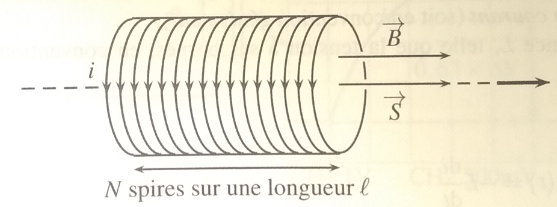
\includegraphics[scale=1]{Lecons_de_physique_2019-2020/Lecons_autres/bobine.png}
%\end{figure}

Importance de l'agébrisation : l'orientation du courant défini l'orientation des surfaces.
On calcule le flux propre dans le cas où l'on suppose que le champs$\overrightarrow{B}$ créé par la bobine est celui d'un solénoide infini.
Le calcul du flux à travers une spire, puis $N$ spires donne
\begin{equation}
\Phi_B = \frac{\mu_0 N^2 S i}{l}
\end{equation}
En appliquant la loi de Faraday, on trouve
\begin{equation}
e = -L\frac{\d i}{\d t},
\end{equation}
où $L = \mu_0 N^2 S/l$ est l'inductance de la bobine  
$L$ s'exprime en Henri ($\mathrm{H}=\meter^2\cdot\kilogram\cdot\second^{-2}\cdot\ampere^{-2})$.

Ici la bobine est traitée en convention générateur car elle est assimilée dans le circuit à un générateur.
En convention récepteur, on a l'habitude de travailler avec $U_L = -e$.
(Schémas au tableau des deux circuits dans chacune des deux conventions, avec la bobine et une résistance $R$ en série.)

L'énergie stockée dans la bobine est liée à son inductance et se trouve en exprimant la puissance électrique qui parcourt la bobine :
\begin{equation}
{\cal{E}} = \frac{1}{2}Li^2
\end{equation}

\begin{remarque}
L'énergie stockée dans la bobine se retrouve aussi en calculant l'énergie volumique magnétique $B^2/2\mu_0$ et en multipliant par le volume de la bobine.
\end{remarque}

\begin{experience}
Vérification de la dépendance en $N^2$ de l'inductance de plusieurs bobines en mesurant l'inductance d'après la fonction de transfert d'un circuit RL :
\begin{itemize}
\item mesure de l'inductance de quatre bobines de même géométrie mais avec des nobres de spires différents (125, 250, 500 et 1000 spires).
Une mesure est réalisée devant le jury.
\item il est nécessaire de mesure $R$ à chaque fois car la résistance dépend de la longueur de fil de la bobine. Cette mesure est réalisée précisément à l'aide d'un multimètre Keithley permettant de faire une mesure à quatre points.
\item la mesure de $L$ se fait en déterminant la fréquence de coupure du filtre passe bas du premier ordre $RL$.
Pour cela on mesure le rapport entre la tension $U_R$ et la tension du GBF, et on réalise l'acquisition pour différentes fréquences à l'aide du programme python dédié à la mesure de diagramme de Bode.
\item en ajustant sur Qtiplot la courbe obtenue par le modèle analytique $||H(\omega)|| = \frac{1}{\sqrt{1+(\omega/\omega_c)^2}}$, on en déduit $L$ (connaissant $R$) car $\omega_c = R/L$.
\item les différentes valeurs de $L$ obtenue sont ajustée en fonction du nombre de spire par un modèle $\mu_0N^\alpha S/L$ et on obtient bien $\alpha\approx2$.
\end{itemize}
Comparaison entre les valeurs mesurées et les valeurs déduites de la géométrie des bobines.
\end{experience}

\begin{transition}
Regardons ce qui se passe maintenant dans le cas de l'expérience de Faraday, avec deux bobines.
\end{transition}

\subsubsection{Inductance mutuelle 25'}

Schéma de deux bobines d'inductance $L_1$ et $L_2$, parcourue par des courants $i_1$ et $i_2$.
L'inductance mutuelle traduit le couplage entre les deux circuits :
\begin{equation}
e_2 = -L_2\frac{\d i_2}{\d t} - M\frac{\d i_1}{\d t}
\end{equation}

\begin{remarque}
\begin{itemize}
\item le signe de $M$ dépend de l'orientation des deux circuits ;
\item on montre que $M_{12}$ = $M_{21}$ : le résultat est presque immédiat en passant par le potentiel vecteur (démo dans \cite{Perez2009} par exemple).
\item l'énergie d'un système de deux inductance couplées par une mutuelle est donnée par 
\begin{equation}
E_\mathrm{tot} = \frac{1}{2}L_1 i_1^2 + M i_1 i_2 + \frac{1}{2}L_2 i_2^2
\end{equation}
\end{itemize}
\end{remarque}

L'inductance mutuelle traduit le fait qu'il est possible de transférer de l'énergie d'un circuit à l'autre.

Traiter le cas du transformateur : faire le calcul de $i_1/i_2$ avec le théorème d'Ampère et déduire la relation en tension par conservation des puissances.
Une application importante de cet effet est le transformateur, nécessaire au transport de l'énergie à haute tension pour diminuer les pertes dues au transfert (les pertes par effets Joule sont proportionnelles au carré de l'intensité.
En travaillant avec des tensions très élevées ($\sim \unit{400}{\kilo\volt}$), il est possible de transporter des puissances importantes sans avoir un courant important.
On a $P_J = Ri^2 = U^2/R$, mais le $U$ ici correspond à la différence de potentiel entre les deux extrémités du fil électrique, et pas aux $\unit{400}{\kilo\volt}$ qui est la différence de potentiel entre le cable et la terre.)
Le transformateur est utilisé pour abaisser la tension en vue d'une utilisation par les particuliers.

\begin{transition}
Après l'induction de Neumann, on va s'intéresser à l'induction de Lorentz, c'est à dire à un circuit mobile.
\end{transition}

\subsection{Induction de Lorentz (circuit mobile) 28'30}

\subsubsection{Rail de Laplace}

Deux termes : 
\begin{itemize}
\item force électromotrice : elle traduit le couplage mécanique $\rightarrow$ électrique ;
\item force de Laplace, responsable du couplage électrique $\rightarrow$ mécanique.
\end{itemize}
Schémas du dispositif, mécanique et électrique.

Avant la mise en équation, on peut qualitativement déterminer l'évolution du système lors d'un déplacement de la tige avec la loi de Lenz (...).
Mise en équation :
\begin{itemize}
\item équation électrique
\begin{equation}
Ri = -vlB
\end{equation}
\item équation mécanique : principe fondamental de la dynamique projeté selon x
\begin{equation}
m\dot{v} = ilB
\end{equation}
\end{itemize}
La résolution de ce système donne 
\begin{equation}
v = v_0 e^{-t/\tau}
\end{equation}
où $\tau = \frac{mR}{B^2 l^2}$.
La barre est ralenti, ce qui est en accord avec l'analyse qualitative avec la loi de Lenz.
Si l'on souhaite arrêter complètement la barre, il faut rajouter un frottement mécanique.

Conversion électromécanique :
Schéma des échanges ($P_{laplace}$ et $P_{induction}$) pour faire le lien entre les pertes par effet Joule et la variation d'énergie cinétique.
On a $P_{laplace} + P_{induction} = 0$

\begin{slide}
Freinage par induction utilisé pour les poids lourds ou encore les trains (présente l'avantage de ne pas nécessité de pièce d'usure).
Les courants créés dans la masse métallique sont appelés courants de Foucault.
Une autre application de l'induction de Lorentz est la roue de Barlow qui peut être utilisée comme générateur de générateur de courant continu (actuellement, cette méthode sert encore pour générer les courants intenses nécessaires aux électrolyses).
L'induction est aussi à la base des méthodes de production d'électricité (alternative) actuelles.
\end{slide}

\begin{experience}
Rail de Laplace : le rail a tendance à rester collé sur le support (les faux contacts entre les rails et la tige créent des arcs électriques qui soudent la barre aux rails).
On pourrait ici faire une démonstration qualitative de la roue de Barlow.
\end{experience}

\subsection*{Conclusion 39'}

Au cours de cette leçon, on a vu :
\begin{itemize}
\item les lois de l'induction (Lenz et Lorentz) ;
\item les inductions de Neumann et Lorentz.
\end{itemize}

\begin{slide}
Applications : générateurs, chauffage par induction, micro, chargeur sans fil...
\end{slide}

\begin{slide}
\href{https://www.youtube.com/watch?v=nIFSZfKTUKA}{Railgun de l'espace} pour la blague :)	
\end{slide}


\subsection*{Questions}

\begin{enumerate}
\item Lors de l'approche historique avec l'expérience de Faraday, vous avez parlé de galvanomètre : qu'est-ce que c'est ? Il s'agit d'un instrument permettant de mesurer de faibles courants électriques.
L'aiguille de l'appareil est liée à des spires parcourue par le courant à mesurer, spires placées dans un champ magnétique constant et homogène.
Le dipôle magnétique formé par les spire est alors soumis à un couple qui dévie l'aiguille.
\item Lors de l'introduction des lois de l'induction, vous avez introduit trois ingrédients : force de Lorentz, $\overrightarrow{E} = -\grad V - \d\overrightarrow{A}/\d t$ et $\overrightarrow{v}\wedge\overrightarrow{B}$ : Commenter ces termes. La force de Lorentz permet d'expliquer comment le champ electromagnétique peut mettre en mouvement ou dévier des particules chargées.
On repart des équations de Maxwell pour exprimer $\overrightarrow{E}$ en fonction des potentiels vecteur et scalaire.
\item Que représentent $V$ et $\overrightarrow{A}$ ?
voir le cours d'électromag de Jérémy pour des discussions plus poussées.
On ne peut pas mesurer directement ni l'un ni l'autre.
On a seulement accès à des différences de potentiel ou à la circulation de $\overrightarrow{A}$.
Dans le cas d'un solénoide parfait avec une spire autour, le champ $\overrightarrow{B}$ est nul au niveau de la spire pourtant il est possible de crée un fem dans la spire en faisant varier le courant dans le solénoïde (le champ $\overrightarrow{B}$ est bien nul mais pas $\overrightarrow{A}$ au niveau de la spire).
Une autre expérience mettant en évidence le rôle de $\overrightarrow{A}$ dans la compréhension d'effets subtils est celle d'Aharonov-Bohm.
\item Comment pourrait-on préciser l'introduction de la force électromotrice $e$ ? Lien entre le travail et la ddp (le travail de la force de lorentz permet d'introduire la ddp)
\item Dans la force de Lorentz, Que représente $\overrightarrow{v}$ ? C'est la vitesse des porteurs de charge.
\item Quel est le référentiel dans lequel est défini $\overrightarrow{v}$ ?
\item vitesse du circuit = vitesse des charges ?
Ici il faut utiliser la composition des vitesses :$\overrightarrow{v} = \overrightarrow{v_{circuit}} + \overrightarrow{u}$, où $\overrightarrow{v_{circuit}}$ est la vitesse du circuit dans le référentiel du laboratoire et $\overrightarrow{u}$ est la vitesse des électrons dans le référentiel lié au circuit.
Quand on considère l'effet d'un champ magnétique sur les électrons, on peut alors considérer le cas d'un conducteur filiforme : la vitesse $\overrightarrow{u}$ étant alors toujours colinéaire avec le conducteur, seule la vitesse des électrons liée au mouvement du circuit donne lieux à une circulation non nulle ($\overrightarrow{u}\wedge\overrightarrow{B}$ est toujours orthogonal au conducteur).
Dans le cas d'un conducteur ayant une section finie, le déplacement de électrons le long du circuit donne en présence d'un champ magnétique l'effet Hall qui est négligeable dans les conducteur en raison de la densité importante de porteurs de charge.
\item Comment évolue la vitesse de chute de l'aimant en fonction du matériau du tube ? Plus le matériaux est conducteur, plus le freinage est efficace, donc la chute longue.
\item Justifier l'approximation du solénoïde infini pour les bobines ?
Cette approximation est sans doute discutable car : les bobines utilisées sont de section carrée et la dimension de la section est comparable à la longueur de la bobine.
Cependant, même dans le cas d'une simple spire, le champ créé en dehors de l'axe est compliqué à calculer.
Les résultats obtenus lors des expériences étant en accord raisonnable avec le modèle simple d'un champ uniforme, on peut ici justifier l'utilisation de cette approximation.
\item Pourquoi sommer les champs $\overrightarrow{B}$ ? On peut appliquer le principe de superposition associé à la linéarité des équations de Maxwell.
\item Pourquoi se placer en convention générateur ? Dans le cas de l'induction présenté ici, la bobine est la source de la force électromotrice.
Il s'agit d'un générateur qui justifie l'emploi de la convention associée. 
\item Puissance stockée dans la bobine. Pourquoi $iU_L$ et pas $ei$ ? Lié à la convention choisie : en convention générateur, on considère l'énergie cédée par la bobine au circuit.
En convention récepteur, on s'intéresse à l'énergie reçue par la bobine.
\item Manip : Quelle est la valeur de la résistance de la bobine et justifier le choix de la résistance ?
(dépend du nombre de spires de la bobine) Il faut que la résistance de la bobine reste faible devant la résistance placée en série avec la bobine.
De plus, on fait en sorte que la fréquence de coupure du passe base soit de l'ordre de \unit{10}{\kilo\hertz} 
\item D'où viennent les incertitudes sur la mesure ? Comment sont calculées les erreurs ? Lors de la mesure de la fréquence de coupure, l'incertitude vient de l'ajustement des données expérimentales par le modèle analytique.
La déduction de $L$ dépend aussi de la valeur de la résistance $R + r$ qui est mesurée précisément avec l'ohmmètre numérique et une mesure à quatre points.
Cette incertitude est données par la notice de l'appareil.
\item Est-il possible de rajouter des erreurs sur les points acquis à l'oscilloscope à la main ?
Oui en se référant à la notice de l'instrument mais elles sont petites venant de l'oscilloscope.
\item Pourquoi avoir choisi de mesurer $L$ d'après le diagramme de Bode ?
Essentiellement car il faut une mesure quantitative dans la leçon docteur.
Autres méthodes : umax/2, temps de montée, etc.
Justifiée par une approche pédagogique.
\item Valeur d'inductance comparée à quoi ? A celle mesuré au RLC-mètre, à la valeur annoncée par le constructeur, à la valeur attendue compte tenu du modèle.
\item D'où vient l'incertitude sur l'inductance théorique ? Principalement de l'inhomogénéité du champ $\overrightarrow{B}$ dans toutes les spires et sur toute la surface d'une même spire.
\item Inductance mutuelle ? pourquoi mettre des dérivée ronde ? (erreur)
\item Une seule équation : couplage de 1 vers 2. Qu'est ce qui se passe dans l'autre sens ?
Le problème est symétrique.
\item L'inductance mutuelle est elle la même de 12 ou 21 ? Oui.
\item Équivalence des puissances de Laplace et induit ? Oui car sinon fuck la physique.
\item Roue de Barlow pour générer du courant ? Oui pour les forts courants de certaines électrolyses, non pour la production électrique actuelle (alternateurs).
\end{enumerate}

\subsection*{Commentaires}

Point noir de la leçon : comment amener les lois de l'induction ?
On peut écrire que la vitesse des électrons est la composition des électrons dans le circuit + la vitesse du circuit.
Une autre possibilité serait de faire l'approche historique entière et introduire le dphi directement.
Bq d'applications : bien
A n'est pas mesurable car il y a une jauge près mais ddp mesurable et la circulation de A aussi.
\newpage